
\section{Introduction}

The demands of everyday life require us to flexibly shift our attention between many different aspects of the visual world. When researchers operationalize these behaviors they often turn to tasks in which an observer must select information from the visual scene either from a spatial location, a particular feature dimension, or combinations of these. The intuitive difference between spatial location and other features has led to categorizing covert visual attention into two types: spatial attention, when task demands require selecting information at a specific location and not others, and feature-based attention, where task demands require selecting particular features (e.g. colors, spatial frequencies, motion directions, etc). This categorization may reflect a real physiological difference in how spatial and feature-based attention are implemented by the brain. It is also possible that space is not privileged over other features in visual cortex, and that instead, selection of information is a generic computation.

Although the majority of attention research has focused on isolating feature-based attention from spatial attention \citep{Saenz2002-fs}, occasionally researchers have focused on comparing the two forms of selection. Previous psychophysics research has shown that selection by location may be slightly faster than selection by feature \citep{Liu2007-ed} [todo: cite harter 1982, hillyard munte 1984] and that spatial selection may be primary \citep{Soto2004-cs,Tsal1988-qx}. The idea of primacy has been shown by showing that subjects are more likely to recall letters near an attended location in space over letters of a similar color at distant locations \citep{Tsal1988-qx} and that errors in letter recall occur for spatial neighbors but not for color-matched distant neighbors [todo: cite snyder 1972]. Another way this has been described is to say that stimuli must be bound together by location to create objects \citep{Treisman1980-gu}, making location primary over other features. Other comparisons have suggested that spatial attention might have more of an influence on perceptual sensitivity and that small differences in stimulus noise have different effects on spatial vs. featural selection \citep{Ling2009-rq}.

To separate spatial and feature-based attention we built a stimulus in which different forms of selection could be compared. We used this stimulus in two tasks, a perceptual averaging task and a working memory estimation task. In both tasks observers were asked to select information either by spatial location or according to a stimulus property (either motion direction or color) while reporting about a third property. In both data sets we show that sensitivity is extremely similar between each form of selection and that any differences in performance are accounted for by changes in bias to the irrelevant dot patches. Finally, we suggest possible implementations by which a common computation could select sensory representations and account for the behavioral observations. 

\section{Methods}

\subsection{Observers}
In total 13 observers were subjects for the experiments. All observers except one (who was an author) were naive to the intent of the experiments. One observer was excluded during the initial training sessions due to an inability to maintain appropriate fixation (see eye-tracking below). Procedures were approved in advance by the Stanford Institutional Review Board on human participants research and all observers gave prior written informed consent before they participated in the experiment. When necessary, observers wore corrective lenses to correct their vision to normal. Observers were filtered prior to inclusion based on self-reported color vision and tested for colour vision deficits using the Ishihara test (color-blindness.com), one observer had to be excluded based on the test results. 

\subsection{Hardware setup for stimulus and task control}

Visual stimuli were generated using MATLAB (The Mathworks, Inc.) and MGL \citep{Gardner2018-uq}. Stimuli were displayed on a 22.5 inch VIEWPixx LCD display (resolution of 1900x1200, refresh-rate of 120 Hz) and responses collected via keyboard. Output luminance and spectral luminance distributions were measured for the LCD display with a PR650 spectrometer (Photo Research, Inc.). The gamma table for each display was dynamically adjusted at the beginning of each trial to linearize the luminance display such that the full resolution of the 8-bit table could be used to display the maximum contrast needed. The luminance spectra were used to compute a transformation matrix from the L*a*b* color space to the RGB output of the screen, such that the a* and b* dimensions could be separately manipulated without changing the luminance (L*). Other sources of light were minimized during behavior. Observers used a circular volume controller to submit their responses in angle space (Powermate USB, Griffin Audio).

\subsection{Eye tracking}

Eye-tracking was performed using an infrared video-based eye-tracker at 500 Hz (Eyelink 1000; SR Research). Calibration was performed throughout each session to maintain a validation accuracy of less than 1 degree average offset from expected using a thirteen-point calibration procedure. Trials were initiated by fixating the central cross for 300 ms and canceled on-line when an observer’s eye position moved more than 1.5 degree away from the center of the fixation cross for more than 300 ms. During training and before data collection observers were excluded from further participation if we were unable to calibrate the eye tracker to an error of less than 1 degree of visual angle or if their canceled trial rate did not drop to near zero.

\subsection{Experimental design}

\subsubsection{Averaging task}

Stimuli consisted of two pairs of dot patches, to the left and right of a central fixation cross (0.5 x 0.5 deg). The dot patches were circular regions centered 8 degrees eccentric with a diameter of 10 deg, covering from 3 to 13 deg along the horizontal axis and -5 to +5 deg along the vertical axis. Each patch was filled with two sets of moving dots (0.2 dots / deg$^2$, per set, 0.3 deg diameter). Dots within a patch were given an identical color (equal luminance, with a* and b* varying) and moved in the same direction at 3.5 deg / s. Dots were `alive' for 0.25 s before vanishing and reappearing immediately at a new random location.

On each trial in the averaging task observers were asked to report the average motion direction of two dot patches (Fig. \ref{fig:c4f1}. Before each set of 20 trials observers were told which feature they would be selecting the patches with with the phrase ``cue side'' or ``cue color'' shown at fixation. Each trial was initiated by the observer fixating the central cross for 300 ms. This was followed by a 0.75 s cue, either a line to the left or right or a miniature patch of colored dots. The feature instructed the observers about which two dot patches they would need to average: either the two on the left, on the right, or the two yellow or blue patches (one on the left and one on the right). A 0.75 s delay followed. During the stimulus period the dot patches began moving coherently in random directions. The target patches were constrained to be less than 135 degrees apart, to avoid confusion about the correct response (e.g. when 180 degrees apart, two possible answers are correct). Observers were shown the stimulus for a variable duration of 0.25 to 0.75 s, then allowed unlimited time to rotate the response wheel and make a response. Feedback was given by showing the actual average motion direction (see Figure). Each trial was followed by a brief inter-trial interval (0 - 2 s, uniformly distributed).

\subsubsection{Psychophysical distance}

We report all of our results according to the normalized psychophysical distance between angles in motion direction and color space, rather than the physical units. Our motivation for this is based on a recent result showing that in working memory estimation tasks, correctly taking into account the psychophysical distance is critical to correctly interpreting data [todo: cite schurgin]. In brief, the motivation for this scaling is that beyond a certain degree distance the ``psychophysical'' distance becomes compressed. The intuition here is that if you are trying to compare N and NE to E, it's easy to tell that NE and E are closer. But if you are trying to quickly compare N and NE to S, this task is more difficult and there is little difference between that comparison and N and NE to SW. Without this re-scaling of distances it's easy to mistake poor sensitivity for a high lapse rate. The authors of [todo: cite schurgin] convincingly demonstrate that in fact lapse rates are consistently low in difficult working memory tasks. Once scaling is taken into account a single sensitivity parameter captures a multitude of effects. For our purposes we approximated this scaling by fitting a sigmoidal function to data available in that paper: 

\begin{equation}
    d(x) = 1.1\frac{x^{1.5}}{x^{1.5}+35^{1.5}}
    \label{eqn:c5psycho}
\end{equation}

Where $d$ is the normalized distance and $x$ is the angular distance in degrees. 

\subsubsection{Estimation task}

On each trial in the estimation task observers were asked to report about either the color or motion direction of a single dot patch. Before each block of 40 trials observers were told which feature would be reported with either the phrase ``report color'' or ``report direction'' appearing on the screen. Key to the task was that although observers ultimately reported about only one dot patch they could be cued to remember just that patch, or multiple patches, during a brief delay period. Each trial consisted of the following sequence: a fixation period [todo]

\subsubsection{Estimation task data analysis}

To analyze the results of the estimation task we fit a modified version of the target confusability competition model from [todo: cite schurgin]. The model is based on the idea that noisy internal channels are independently competing to represent a stimulus (Fig. \ref{fig:c4f4}a). On each trial the model proceeds in two steps. First, the stimulus (or stimuli) are encoded by the channels, setting their mean response. The profile of each channel comes from a re-scaling of the angle (in a* b* space, or in motion direction space) to the normalized psychophysical distance (Eq. \ref{eqn:c5psycho}). As an example of the encoding step the response of a small set of channels (Fig. \ref{fig:c4f4}a) to a stimulus with an angle of zero are shown (Fig. \ref{fig:c4f4}b). Therefore, each channel response is distributed as follows:

\begin{equation}
    C_{\theta}(x) = \mathcal{N}(\mu = \alpha(x-\theta),\sigma=1)
    \label{eqn:c5channel}
\end{equation}

Where $\theta$ is the preferred orientation for that channel. $\alpha$ is an amplitude parameter which controls the scaling of the response and is the only free parameter in the model.

The second step in the model is to find the observer's behavioral response by taking the maximum response among the channels. Because each channel has independent normally-distributed noise, the likelihood of each channel winning this can be computed as the conditional probability of a channel exceeding all of the other channels. We approximate this likelihood by computing the likelihood over all possible channel responses, as follows:

\begin{equation}
    \matchcal{L}(\theta) = \int_{-\infty}^{\infty} P(x_{\theta}=a) \prod_{j\neq \theta}(P(x_j < a)) da
    \label{eqn:c5like}
\end{equation}

Where $P(x)$ is normally distributed with $\mu=0$ and $\sigma=1$. To compute the full likelihood distribution we evaluate Eq. \ref{eqn:c5like} at all values of $\theta$.

Because the response calculation is analogous to signal detection the $\alpha$ parameter in Eq. \ref{eqn:c5channel} is actually the sensitivity of the channel (i.e. $d'$). We can fit this free parameter to a data set by maximizing the likelihood of observed responses to obtain an estimate of the perceptual sensitivity.

We performed the model fitting step in such a way as to separate an observer's bias (i.e. likelihood of responding about the incorrect dot patch) from their sensitivity (i.e. their variability in response quality, for a given dot patch). We did this by modeling the observer's trial-by-trial response as a combination of a likelihood function for each stimulus patch (Eq. \ref{eqn:c5like}) with a set of bias parameters.

\begin{equation}
    \matchcal{L}(\theta) = \beta_{target}\matchcal{L}_{target} + \beta_{side}\matchcal{L}_{side} +\beta_{feature}\matchcal{L}_{feature} +\beta_{distractor}\matchcal{L}_{distractor}
\end{equation}

Where the terms target, side, feature, and distractor correspond to the dot patches that are on the same side, opposite-side with matched-feature, and opposite-side with mismatched-feature, respectively (Fig. \ref{fig:c4f5}). The actual $\beta$ values were constrained so that $\beta_{target}+\beta_{side}+\beta_{feature}+\beta_{distractor}=1$, by calculating them from intermediate values:

\begin{equation}
    \beta_{target} = \beta_{s} * \beta_{f}
\end{equation}

\begin{equation}
    \beta_{side} = \beta_{s} * (1-\beta_{f})
\end{equation}

\begin{equation}
    \beta_{feature} = (1-\beta_{s}) * (1-\beta_{d})
\end{equation}

\begin{equation}
    \beta_{distractor} = (1-\beta_{s}) * \beta_{d}
\end{equation}

Where $\beta_s$, $\beta_f$, and $\beta_d$ are each constrained to the range [0,1]. In this way, setting $\beta_s=1$ and $\beta_f=1$ means that the observer is always choosing the target and never incorrectly reporting about the other three dot patches (i.e. $\beta_{target}=1$).

In sum, we fit four sensitivity parameters ($\alpha$) and three bias parameters ($\beta$) for the data set in which observers selected by location or color and separately for the data set in which they selected by location or motion direction.

\subsection{Implementing attention in a channel linking model}

The channels in the behavioral model described above have tuning which, by definition, matches the behavior. In reality, the psychophysical scaling is a result of the readout process from neurons tuned with much sharper functions. To explore how attention might change channel responses we explored how to connect sharp tuning functions, such as those neurons might have, to the psychophysical space described above. One way to approach this problem is to assume that the psychophysical similarity is the result of correlating channel response profiles which have exponential decay (M. Schurgin, personal communication, 2019). But neural tuning functions have a variety of profiles and restricting them to only exponential distributions is too restrictive. In our simulations we avoided this issue by assuming that the psychophysical similarity is a side effect of a readout process, rather than a function of that process.

In our simulation we assumed that channels had a Von Mises tuning with a relatively sharp profile (Fig. \ref{fig:c4f7}a). The Von Mises distribution is computed from the equation:

\begin{equation}
    \exp(\frac{\kappa*\cos{x-\mu}}{2*\pi*I_0(\kappa)})
\end{equation}

The parameters $\mu$ and $\frac{1}{\kappa}$ are analogous to $\mu$ and $\sigma^2$ of the normal distribution. $I_0$ is the modified Bessel function of order 0.

As before the response of each channel had independent Gaussian noise at the time of stimulus encoding. To read out from these channels we assumed there were a large number of parallel linear readouts. Each linear readout was assigned a single stimulus value (e.g. $\theta=0$) and computed the dot product of the channel responses (with noise) against the ideal response of each channel for that stimulus value in the absence of noise. We assumed that the choice of the entire system would be the stimulus value with the maximal dot product response.

[todo: not sure how to format equation]

% \begin{equation}
%     \max_{\mu}
% \end{equation}

To simulate different models of attention we either applied a gain to the noisy channel responses or changed the set of mean channel tuning values. 

\section{Results}

\begin{figure}
\centering
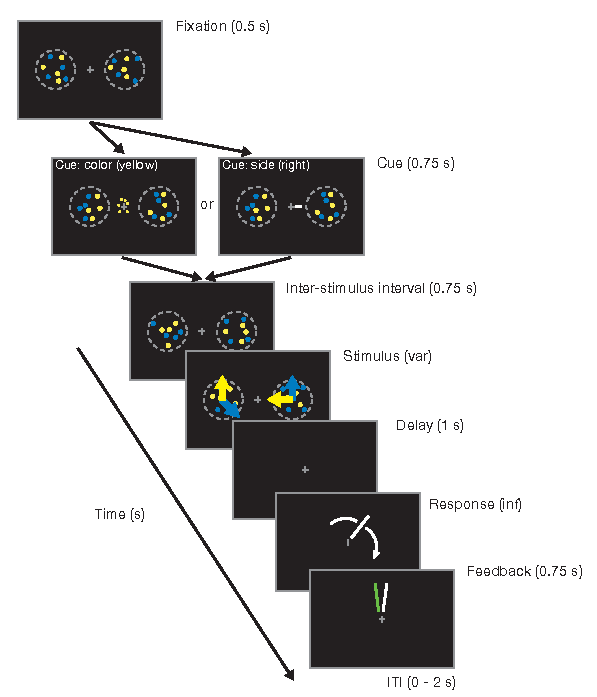
\includegraphics[keepaspectratio,width=0.5\textwidth]{figs_c4/f1_task.pdf}
\caption[Averaging task]{Motion direction averaging task. Observers were asked to select two out of four random dot patches and average their motion direction. Observers initiated trials by fixating a central cross, causing the two dot patches to appear with incoherent motion. A cue indicated whether they should select the left or right patches (spatial selection) or the yellow or blue ones (feature-based selection). After a brief delay the dot patches each began moving in random directions, before vanishing again for a second short delay. Finally, observers used a rotating wheel to report the \textit{average} direction of motion for the two dot patches they were asked to select. Feedback was given by indicating the true average motion direction.}
\label{fig:c4f1}
\end{figure}

We characterized human perceptual sensitivity to the average motion direction of two dot patches, while asking observers to select the two patches either based on their common location or a shared feature (Fig. \ref{fig:c4f1}. To measure perceptual sensitivity we recorded each observer's estimation error relative to the true average motion direction. We found that whether observers selected the two dot patches by spatial location (left or right) or by feature (yellow or blue), their estimation errors remained nearly identical (Fig. \ref{fig:c4f2}). Consistent with the task design we found that giving observers a longer stimulus (Fig. \ref{fig:c4f3}a) or a smaller angle difference between the two dot patches (Fig. \ref{fig:c4f3}b) improved sensitivity slightly. 

\begin{figure}
\centering
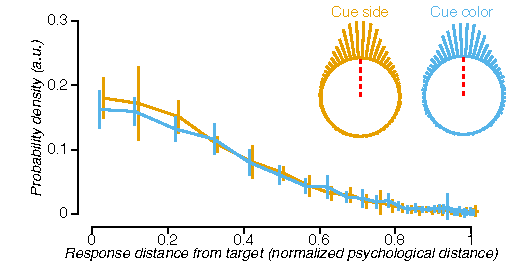
\includegraphics[keepaspectratio,width=0.5\textwidth]{figs_c4/f2_aca_perf.pdf}
\caption[Estimation error during averaging]{Estimation error during the averaging task. A histogram displaying the average proportion of responses at each distance from the true average motion direction (0) is shown, averaged across observers. Selection by spatial location (i.e. averaging the two patches on the right or left) is shown in yellow, and selection by color (i.e. averaging the two yellow or blue patches) is shown in blue. The two inset plots show the same histogram but in a circular space, with a red dashed line indicating the true average. Note that the x-axis has been re-scaled from degrees to psychophysical distance, see Methods for details.}
\label{fig:c4f2}
\end{figure}

\begin{figure}
\centering
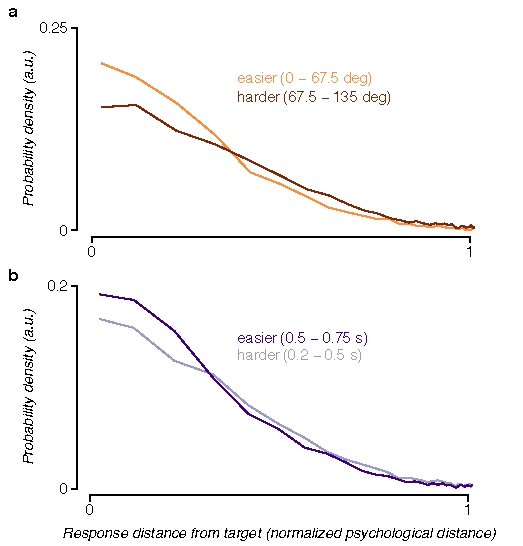
\includegraphics[keepaspectratio,width=0.5\textwidth]{figs_c4/f2_aca_parameters.pdf}
\caption[Parameters that control difficulty of averaging]{Averaging difficulty is controlled by stimulus duration and angle distance between patches. (a) The average estimation error across observers is shown for a median split of the angle difference between the two dot patches that were averaged. (b) As in (a) for a median split of stimulus duration.}
\label{fig:c4f3}
\end{figure}

The averaging task demonstrates that if differences in selection exist they are small and may depend in specific ways on the context of particular tasks. What that design cannot differentiate is whether any small performance differences are the result of a change in the sensitivity between conditions or bias between conditions. In some previous experiments researchers have reported that spatial compared to feature-based selection leads to small differences in timing \citep{Liu2007-ed} and performance [todo: cite]. We next sought to design a task which could differentiate between changes in bias and sensitivity. Our rationale was that a change in bias should be related to observers making errors, for example by choosing the wrong stimulus to report, whereas a change in sensitivity would be related to the variability in the sensory representation and motor response. We first designed a task to orthogonalize these dimensions and then extended an existing psychophysics model to capture the behavior. 

\begin{figure}
\centering
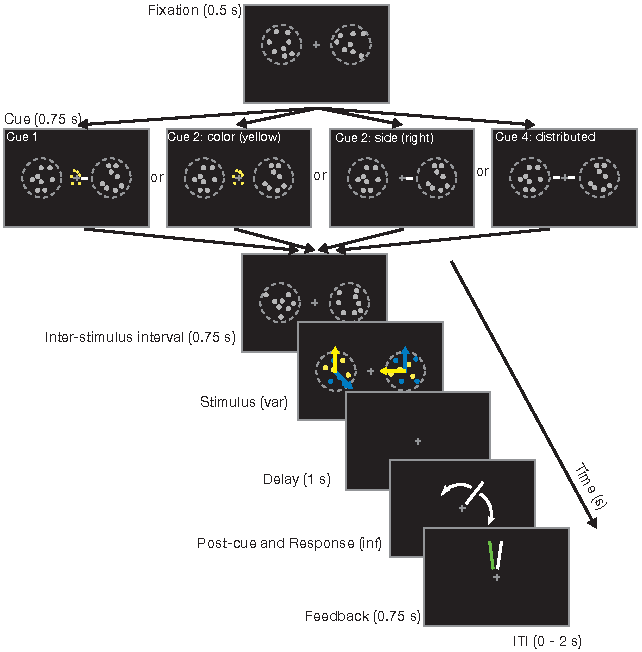
\includegraphics[keepaspectratio,width=0.5\textwidth]{figs_c4/f4_estimationtask.pdf}
\caption[Estimation task]{Estimation task. Observers began each trial by fixating a central cross (Fixation). A pre-cue (Cue) was then shown }
\label{fig:c4f4}
\end{figure}

The estimation task uses the same stimulus as the averaging task, but we now asked observers to recall a single motion direction (rather than the average of two). Prior to reporting this observers could be cued to remember only the direction of motion of the target they would later report, or the motion direction of multiple dot patches (Fig. \ref{fig:c4f4}). In the most difficult case (Cue 4: Distributed) observers memorized the directions of all four potential targets. In two conditions observers were asked to memorize either the motion directions of the two patches on the left or right (Cue 2: side) or the two yellow or blue patches (Cue 2: color), in the same manner as in the averaging task. In all conditions a Post-Cue was used to reveal which of the memorized motion directions had to be reported.

\begin{figure}
\centering
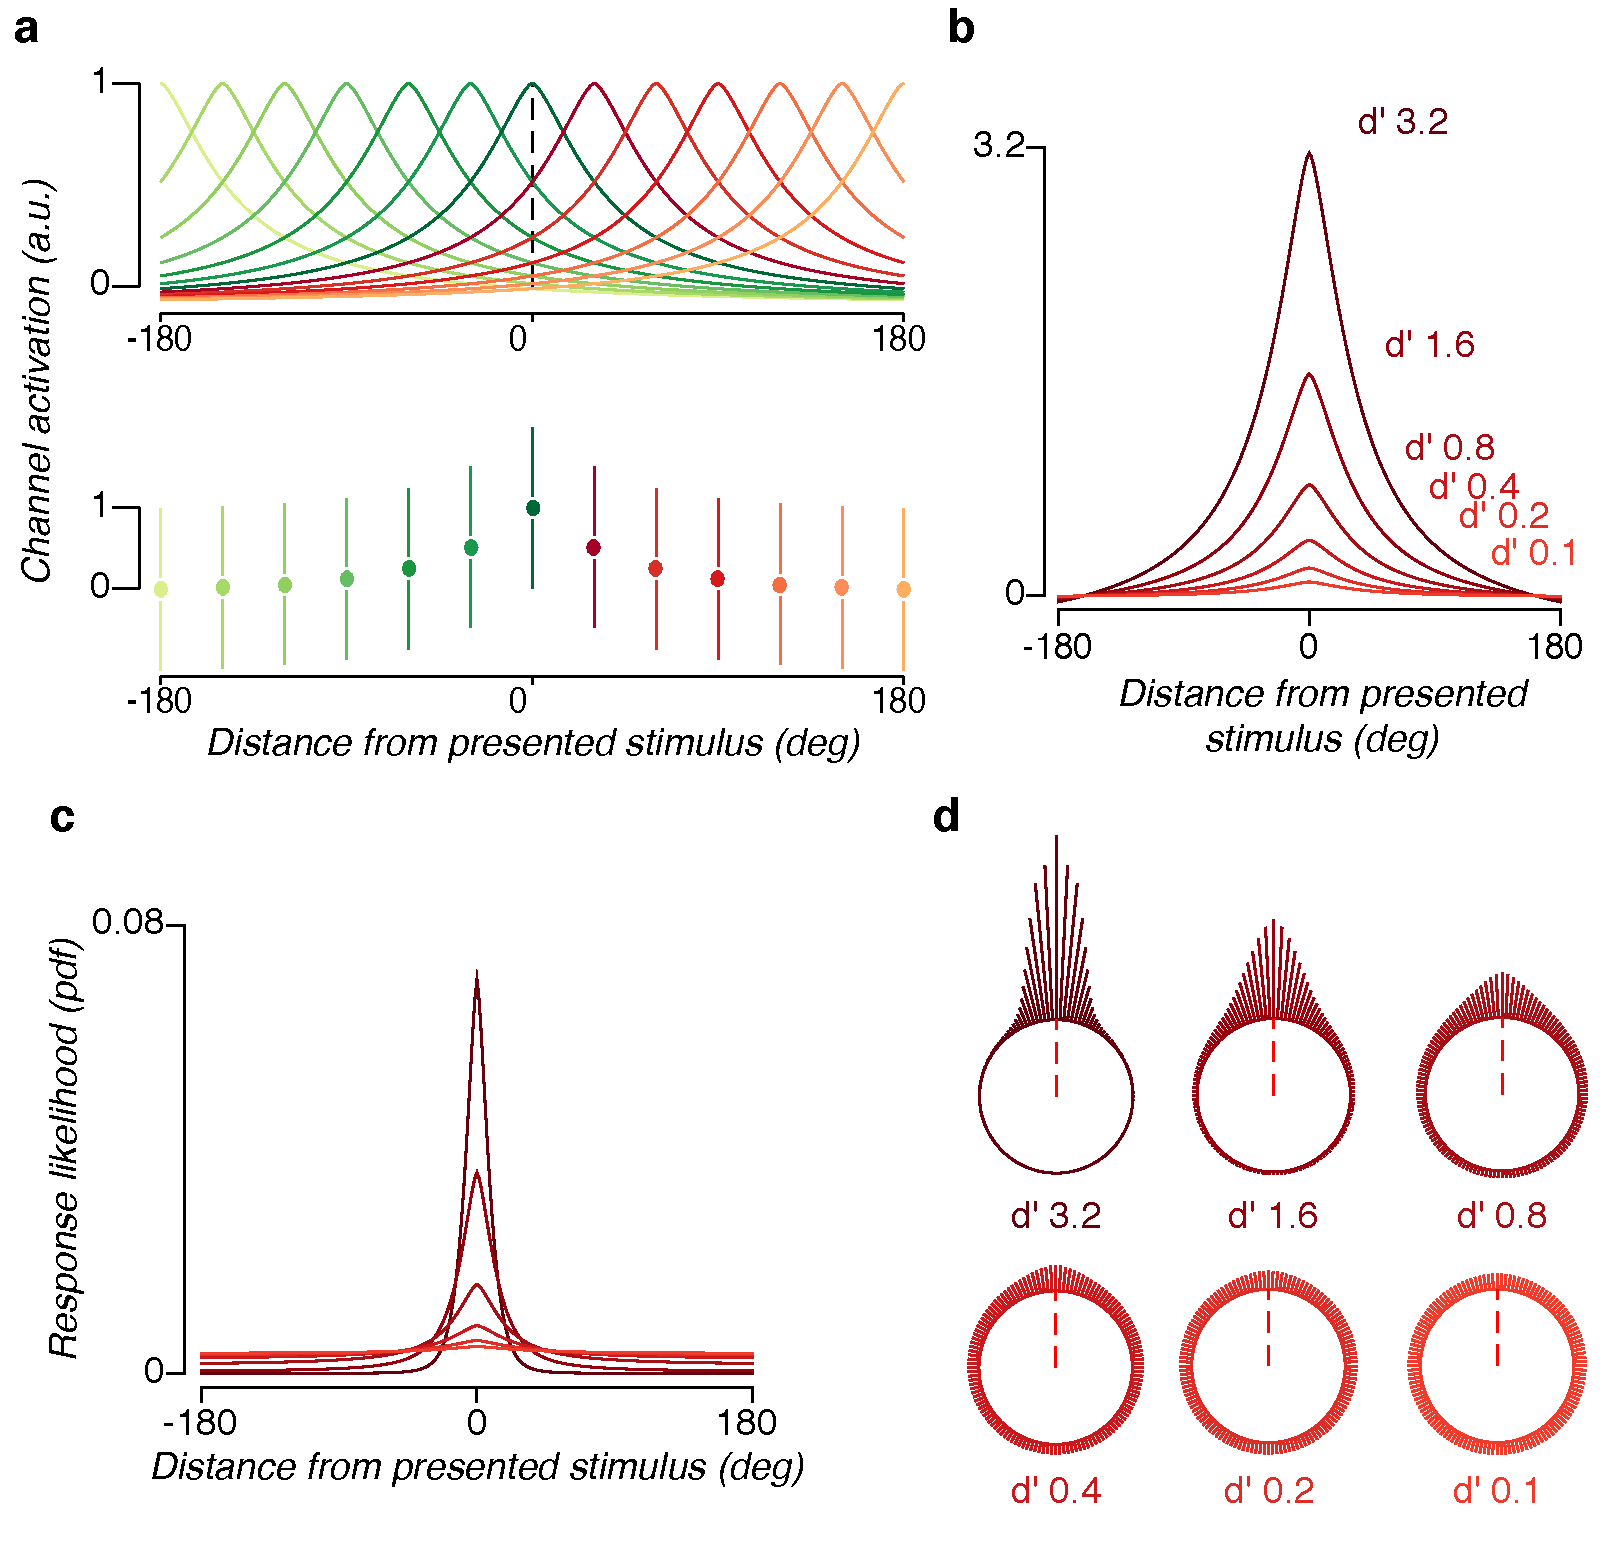
\includegraphics[keepaspectratio,width=0.5\textwidth]{figs_c4/f3_TCC_model.pdf}
\caption[Estimation task model]{Estimation task model. The model of the estimation task is based on an existing model of working memory estimation by \citet{Schurgin2018-vi}. (a) In the model independent channels encode the stimulus with a response profile defined by the psychophysical distance of each channel's preferred response and the stimulus. The channel responses are normally distributed with $\sigma=1$. (b) A free parameter in the model controls the sensitivity of the channels ($d'$), which acts as a multiplicative gain on the amplitudes of each channel response. (c) To read out an estimate of the stimulus angle an observer takes the maximum response over the channels. We show here the full likelihood distribution over all angles, computed numerically (see Methods: todo). (d) The same distributions in (c), the likelihood of response for different values of $d'$, are shown in circular space.}
\label{fig:c4f5}
\end{figure}

To understand the data we collected from the estimation task we needed to decompose bias from sensitivity. To do this we employed a simple model of perceptual sensitivity which fits two parameters for each condition. TODO (Fig. \ref{fig:c4f5}). 

\begin{figure}
\centering
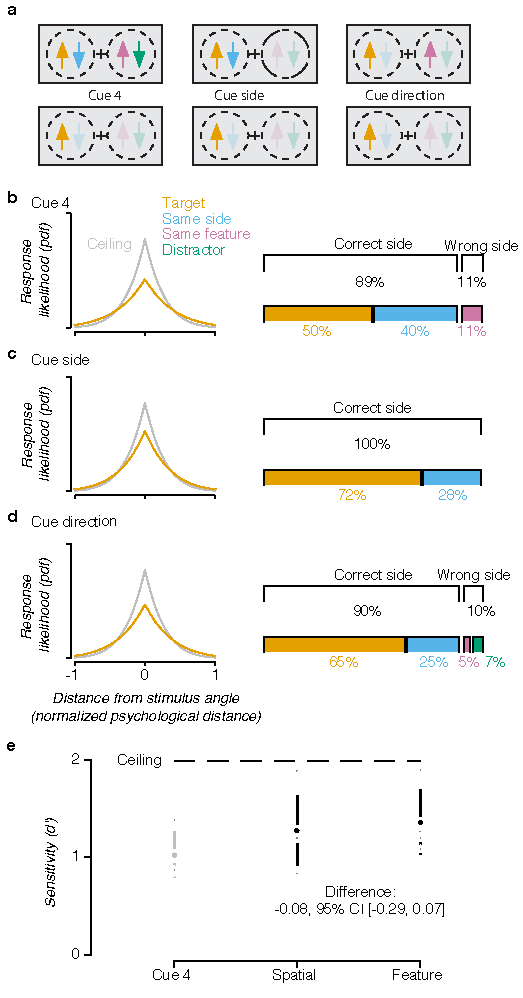
\includegraphics[keepaspectratio,width=0.5\textwidth]{figs_c4/f4b_estimation_perf.pdf}
\caption[Estimation task performance]{Performance in the estimation task. (a) Three of the conditions used in the experiment are shown for trials where selection was performed by the direction of motion and the report was the color. Opacity is used to indicate which dot patches are memorized in each condition and to emphasize that the response in all conditions is identical (reporting the color of a single dot patch). In Cue 4 trials an observer memorized all four colors shown and was then asked to report the color of a single dot patch, e.g. the dots moving upward on the left side (orange arrow, highlighted). In Cue 2 trials the observer either memorized the colors on one side (Cue side) and was post-cued about the direction, or memorized two dot patches moving in the same direction (Cue direction) and was post-cued about the side. (b) The model estimate of sensitivity for each of the four dot patches is shown separated from the probability of reporting about each dot patch. Observers reported about the distractor dot patch less than 2\% of the time. (c-d) Conventions as in (b) for the two cue 2 conditions. (e) Confidence intervals for the $d'$ parameter are shown for each condition.}
\label{fig:c4f6}
\end{figure}

\begin{figure}
\centering
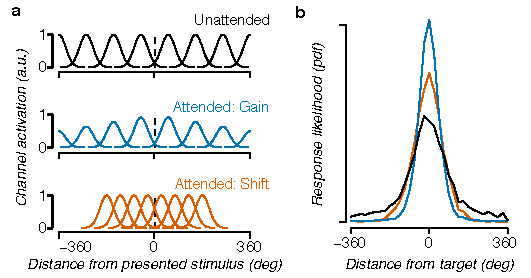
\includegraphics[keepaspectratio,width=0.5\textwidth]{figs_c4/f5_channel_attention.pdf}
\caption[Attention in a channel model]{Implementations of attention in a hypothetical channel model. (a) Examples are shown of how neuron responses might change during attention. (b) Response likelihoods are shown for the different attention models, see Methods for model details.}
\label{fig:c4f7}
\end{figure}

\section{Discussion}



In general, the idea that spatial selection precedes feature-based selection matches in some ways with cortical physiology. Early visual cortex is organized retinotopically \citep{Wandell2007-pr} while sensitivity to specific visual features only emerges later [todo: cite]. 

The stimulus we studied has been used previously to study how feature-based attention occurs in the brain \citep{Saenz2003-qz}. Also \citep{Saenz2002-fs}.